\documentclass[11pt,a4paper]{article}
\usepackage[margin=2.2cm]{geometry}
\usepackage[T1]{fontenc}
\usepackage[utf8]{inputenc}
\usepackage{mathptmx}\usepackage[scaled=.92]{helvet}
\usepackage{microtype}
\usepackage{booktabs,tabularx,array,multirow}
\usepackage{graphicx}
\usepackage{caption}
\usepackage[numbers,sort&compress]{natbib}
\usepackage{url}
\usepackage[colorlinks=true,linkcolor=black,citecolor=blue!60!black,urlcolor=blue!60!black]{hyperref}
\usepackage{xcolor}
\usepackage{amsmath}
\usepackage{enumitem}
\setlist{nosep}
\captionsetup{font=small,labelfont=bf}
\newcolumntype{R}{>{\raggedleft\arraybackslash}X}
\newcolumntype{L}{>{\raggedright\arraybackslash}X}
\urlstyle{same}
\def\UrlBreaks{\do\/\do-\do_\do.\do=\do?\do\%}

\title{\textbf{Public Investment in School Education in Nepal}\\[4pt]\large Government spending per student, FY 2008/09--2026/27: level, composition, trend and variation by government}
\author{Prepared by Claude}
\date{20 October 2026}

\begin{document}
\maketitle

\begin{abstract}
\noindent This paper investigates how much the Government of Nepal invests in school education per student, how that investment is composed, how it has moved since FY~2008/09, and how it compares across the governments that presented each budget. Three findings organise the analysis. First, the correct denominator is community (public) school students only: by statute an institutional (private) school is one approved on condition that it receives no regular government grant, every school-education line in the budget is directed at community schools, and the only fiscal flows between the state and private schools run the other way. On that basis the FY~2026/27 school-education allocation of Rs~151.69~bn works out to about \textbf{Rs~34,600 per community-school student} (Rs~49,800 if the whole education and sports budget is counted). Second, the budget is overwhelmingly a salary budget: roughly 69\% of the education budget is teacher and staff salaries and pensions, and under 5\% is infrastructure. Third, in nominal terms allocation per public-school student has roughly doubled since 2018/19, but in constant FY~2025/26 prices allocation per enrolled student has been flat at about Rs~30,000 since 2019/20; most of the apparent rise per \emph{public} student reflects a 17\% fall in community-school enrolment since 2021/22 rather than more money. The paper also sets out how UNESCO, the OECD and the World Bank define expenditure per student, and places Nepal against its South Asian neighbours on that basis. Every figure is sourced in the reference list.
\end{abstract}

\section{Introduction}
Nepal's constitution promises free education through the secondary level, and successive governments have pledged to devote 20\% of the budget, or 5\% of GDP, to education. This paper asks what that promise amounts to per student. It addresses five questions: (1)~whom the school-education budget actually funds, and therefore what the right denominator is; (2)~what the education budget is made of---how much goes to teachers, to buildings, to school meals, to scholarships and to the other programmes that sit under the education heading; (3)~how much is allocated per student in FY~2026/27; (4)~how that figure has moved since FY~2008/09, in nominal and in constant prices, and how it varies with the government that presented each budget; and (5)~how the measure used here relates to the way UNESCO, the OECD and the World Bank compute expenditure per student, so that Nepal can be placed against its neighbours. All budget figures are initial allocations from the Ministry of Finance as reported in budget speeches, UNICEF and NCE Nepal budget briefs and the press; enrolment figures are from the Ministry of Education's Flash reports and the Economic Survey; every number carries a citation.

\section{Summary of findings}
\begin{itemize}[leftmargin=1.4em]
\item \textbf{Headline, FY 2026/27 (2083/84).} School-education allocation Rs~151.69~bn \cite{radionepal2026} $\div$ 4,383,655 community-school students (Economic Survey 2082/83) \cite{kp2026es} $= $ \textbf{Rs~34,604} per public-school student per year (Rs~32,220 excluding the Rs~10.45~bn infrastructure line). Counting the entire Rs~218.30~bn education and sports budget gives Rs~49,799 per public-school student; spreading it over all 7.04~m students gives Rs~31,005, but that last figure is a national average, not a measure of what any student receives (Section~\ref{sec:results}).
\item \textbf{Denominator.} The Economic Survey 2082/83 counts 7.04~m students in grades 1--12 in 2025/26: 4,383,655 (62\%) in 25,623 community schools and 1,387 religious schools, and 2,657,170 (38\%) in 8,941 institutional schools \cite{kp2026es}. Approximations built from school counts and average school size (170 students per community school, 291 per private school, as reported in the press from the Economic Survey \cite{edukhabar2025}) are not needed when the enrolment counts themselves are published, and are sensitive to which year's counts are paired (Section~\ref{sec:enrol}).
\item \textbf{Private schools receive no budget money.} Education Act 2028 s.~2(d3) \cite{eduact1971}; Compulsory and Free Education Act 2075 ss.~21--22, 27, 30 \cite{cfe2018}; ADB (2021): ``institutional (private) schools do not receive public funding'' \cite{adb2021}. Private schools must instead fund 10--15\% free seats themselves and, from FY~2026/27, pay a 3\% Education Equity Fee on fee income \cite{ican2026} (Section~\ref{sec:private}).
\item \textbf{Composition.} Of the Rs~218.30~bn education and sports budget, 68.98\% (Rs~150.59~bn) is salaries and pensions, 69.07\% (Rs~150.79~bn) is executed by local governments as conditional grants that are mainly community-school teacher pay, and 28.81\% (Rs~62.90~bn) is federal, of which 42\% (Rs~26.50~bn) is teacher pensions alone \cite{ratopati2026,ican2026}. The identifiable programme lines are small by comparison: school infrastructure Rs~10.45~bn (4.8\%), midday meals Rs~9.54~bn (4.4\%), scholarships Rs~8.60~bn (3.9\%), teacher training Rs~3.20~bn (1.5\%), smart boards Rs~1.07~bn (0.5\%) \cite{radionepal2026,republica_meals2026,mof2026,khabarhub2026,republica_budget2026} (Section~\ref{sec:composition}).
\item \textbf{International comparability.} UNESCO and the World Bank define government expenditure per student as actual general-government expenditure (current + capital + transfers) at a level of education divided by \emph{all} students enrolled at that level, expressed as a share of GDP per capita; the OECD divides expenditure from all sources by full-time-equivalent students \cite{wb_meta_prim,uis_meta,oecd2023}. On the UNESCO convention Nepal's 2026/27 school allocation is about 9.7\% of GDP per capita per student, against a South Asian average of 10--12\% and a world figure of 16--20\%; the public-school-only measure used here (15.5\%) is a different, more targeted statistic (Section~\ref{sec:intl}).
\item \textbf{Trend.} The education share of the federal budget fell from 16.6\% (2008/09) and a 17.1\% peak (2010/11) to 9.9\% (2017/18) and has hovered at 10--11.6\% since; it is 10.28\% in 2026/27 against a 20\% commitment \cite{nce2020,unicef2020,kpedit2026}. Nominal allocation per enrolled student rose from Rs~5,456 (2008/09) to Rs~31,005 (2026/27); in FY~2025/26 prices, from Rs~16,386 to about Rs~29,500, with essentially all of the real gain occurring before 2019/20 (Figure~\ref{fig:perstudent}).
\item \textbf{By government.} Measured as real allocation per enrolled student averaged over the budgets each government presented, the series climbs steadily from Rs~16,400 (Dahal~I, 2008/09) to Rs~29,900 (Oli~II, 2018/19--2021/22) and then plateaus: Deuba Rs~31,000, Dahal~III Rs~29,900, Oli~III Rs~30,000, Shah Rs~29,500 (Table~\ref{tab:bygov}, Figure~\ref{fig:bygov}). The Shah government's first budget is the largest in nominal terms and the second-smallest education \emph{share} since 2017/18 (only 2018/19, at 10.20\%, was lower).
\end{itemize}

\section{Does the school budget fund private schools?}\label{sec:private}
\subsection{Legal position}
\begin{itemize}[leftmargin=1.4em]
\item \textbf{Education Act 2028 (1971), as amended.} Section 2(d2) defines a \emph{community school} as one that ``will gain regular grant'' from the government; section 2(d3) defines an \emph{institutional school} as one approved ``on condition that they will not get regular grants''. Section 12B(2)(b) obliges institutional schools to \emph{pay into} the Rural Education Development Fund \cite{eduact1971}.
\item \textbf{Constitution of Nepal 2015, Art.~31(2)} guarantees free basic and secondary education ``from the State'' \cite{constitution2015}; the state discharges this through public schools.
\item \textbf{Act Relating to Compulsory and Free Education 2075 (2018).} Free textbooks (s.~21), learning materials for destitute children and laboratory/sports/computer grants (s.~22) are expressly limited to \emph{public} schools. Section 30 directs federal grants to local governments for basic and secondary education by school and student numbers. Section 27(3) obliges private-investment schools to provide free seats for 10\% (up to 500 students), 12\% (500--800) or 15\% ($>$800) of their enrolment, with no reimbursement provision \cite{cfe2018}. The 10\% scholarship floor also appears in the Education Regulations 2059 and is being enforced through local governments in 2026 \cite{kp2026scholar}.
\item \textbf{ADB assessment of school-education financing (2021):} ``institutional (private) schools do not receive public funding''; the federal conditional grant for school education averaged NPR~13,809 per (community-school) student in FY2019, 74\% of it for salaries \cite{adb2021}.
\item \textbf{School Education Bill 2080} proposed tighter regulation of private schools (trust conversion, full scholarships) but lapsed with the dissolution of the House on 12 September 2025 \cite{himalpress2025}; a replacement bill is being drafted by the present ministry \cite{kp2026bill}. Nothing in either draft creates a grant to private schools.
\end{itemize}

\subsection{Budget structure}
The FY~2026/27 education and sports budget of Rs~218.30~bn is 68.98\% salaries and pensions (Rs~150.59~bn); 69.07\% is executed by local governments, 2.12\% by provinces and 28.81\% federally \cite{ratopati2026}. By sub-sector, school education takes 69.49\% (Rs~151.69~bn, including Rs~10.45~bn infrastructure), higher education 11.04\%, management 15.17\%, TVET 2.56\% and sports 1.74\% \cite{radionepal2026}. Teacher salaries alone are Rs~133.8~bn (61.3\% of the education budget) \cite{onlinekhabar2026}. The local-government share is the conditional grant that pays community-school teachers, textbooks, midday meals and scholarships \cite{unicef2022,kp2024dec}. None of these line items is open to institutional schools. The only fiscal flows between the state and private schools run \emph{from} private schools: the Education Act fund contribution and the new 3\% ``Education Equity Fee'' on all fees collected by private educational institutions (Finance Bill 2083/84, s.~16) \cite{ican2026}.

\textbf{Conclusion.} Per-student government spending should be computed over community-school students only. Minor indirect benefits to private schools (government curriculum, NEB examinations, teacher licensing) are unquantified in any source found and are treated as negligible.

\section{Composition of the education budget}\label{sec:composition}
Figure~\ref{fig:composition} cuts the FY~2026/27 education and sports budget three ways, using the Ministry's own breakdown \cite{ratopati2026,radionepal2026,ican2026,unicef2026}. The three cuts overlap: teacher salaries sit inside the local-government conditional grant, which sits inside school education.

\begin{figure}[htbp]\centering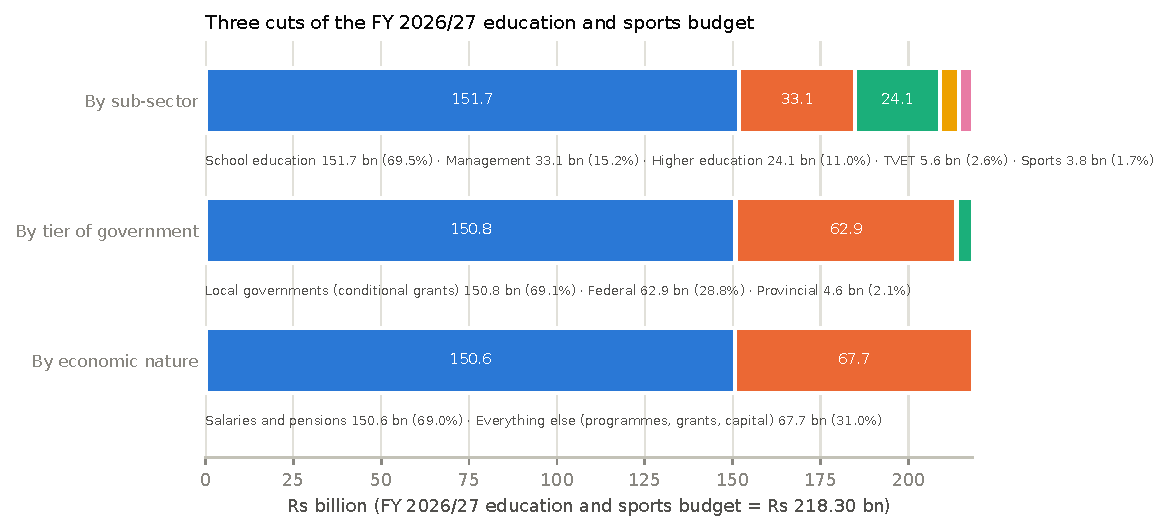
\includegraphics[width=\textwidth]{fig_composition.pdf}
\caption{The FY~2026/27 education and sports budget (Rs~218.30~bn) by sub-sector, by tier of government and by economic nature. Sources: \cite{ratopati2026,radionepal2026,ican2026}; sub-sector amounts other than school education are derived from the published percentages.}\label{fig:composition}\end{figure}

\subsection{Teachers and pensions}
The budget is first and foremost a payroll. Salaries and pensions take 68.98\% (Rs~150.59~bn) of the FY~2026/27 total \cite{ratopati2026}; an NGO-style re-classification puts community-school teacher salaries alone at Rs~133.8~bn (61.3\%) and administrative salaries at Rs~11.5~bn (5.3\%) \cite{onlinekhabar2026,khabarhub2026}. Teacher pensions, paid federally through the Teacher Record Office, are Rs~26.50~bn, 42.13\% of the Rs~62.90~bn federal share, up from Rs~19.00~bn budgeted (Rs~22.18~bn revised) in 2024/25 \cite{ratopati2026,nce2025,kp2024dec}. The 2026/27 budget raised the basic salary scale by 10\% and the teacher grant by 10\%, which the Ministry estimates will require a further Rs~4.69~bn in-year \cite{mof2026,ratopati_pay2026}. In 2024/25, 78.2\% of the local conditional grant (Rs~110.60~bn of Rs~141.36~bn) was teacher salaries \cite{kp2024dec}. ADB's analysis of the FY2019 conditional grant found the same shape: 74\% salaries and allowances, 10\% operations and teaching materials, 9\% school grants and scholarships, 6\% infrastructure \cite{adb2021}. Nearly 90\% of the education budget going to salaries is the figure most often quoted in Nepali commentary \cite{kpedit2026}.

\subsection{Infrastructure}
Physical infrastructure within school education is Rs~10.45~bn (4.8\% of the budget) in 2026/27 \cite{radionepal2026}, of which Rs~2.37~bn is school buildings built in partnership with local governments and Rs~1.00~bn is a national infrastructure-requirement mapping of community schools \cite{republica_budget2026,mof2026}. This is a large step up from Rs~2.5~bn (1,000 classrooms) in 2024/25 and Rs~2.72~bn (completion of model schools) in 2025/26 \cite{edusanjal2024b,edusanjal2025}, but still means that less than Rs~400,000 per community school per year is available for construction and repair.

\subsection{School meals}
The midday meal programme (\emph{diwa khaja}) covers about 2.8~million children from ECED to grade~5 at Rs~20 per child per school day (Rs~25 in Humla, Jumla, Mugu, Dolpa and Kalikot) for 180 days. Its allocation was Rs~8.39~bn in 2024/25 (at Rs~15 per day), Rs~10.19~bn in 2025/26 when the rate rose to Rs~20, and Rs~9.54~bn in 2026/27 \cite{edusanjal2024b,edusanjal2025,republica_meals2026}. It is the largest non-salary programme in school education, at roughly 4.4\% of the budget, or about Rs~3,400 per covered child per year.

\subsection{Scholarships, textbooks and other student-facing grants}
Targeted scholarships from school to higher education are Rs~8.60~bn in 2026/27 \cite{mof2026}, up sharply from Rs~2.44~bn (2025/26) and Rs~0.60~bn for school-level scholarships (2024/25) \cite{edusanjal2025,edusanjal2024b}. Free textbooks for community schools cost Rs~3.81~bn in 2024/25 (2.7\% of the local grant) \cite{kp2024dec}; no separate figure is published for the later years. The 2025/26 budget carried Rs~1.29~bn for free sanitary pads for 1.3~million schoolgirls and Rs~10.16~bn for ECED facilitators and school support staff \cite{edusanjal2025}, whose monthly grants were raised in 2026/27 (ECED facilitators from Rs~12,000 to Rs~17,000) \cite{ratopati_pay2026}.

\subsection{Quality, technology and other programmes}
Teacher mentoring and professional development receives Rs~3.20~bn (1.5\%) \cite{khabarhub2026}; smart boards for every community secondary school Rs~1.07~bn \cite{republica_budget2026}; the President Educational Reform Programme, a federal model-school grant, Rs~0.88~bn (2024/25) and Rs~2.72~bn (2025/26) \cite{edusanjal2024b,nce2025}. Provincial programmes such as SEE management (Rs~35~m) are tiny \cite{republica_budget2026}.

\subsection{Beyond schools: higher education, TVET, sports}
Higher education is 11.04\% of the 2026/27 budget (about Rs~24~bn): the University Grants Commission (Rs~19.7~bn in 2025/26), the Medical Education Commission (government grant Rs~5.99~bn in 2026/27) and the government's Rs~15.63~bn share of Tribhuvan University's Rs~30.87~bn budget are the main items \cite{ratopati2026,nce2025,ekantipur_mec2026,ratopati_tu2026}. Technical and vocational education is 2.56\% (about Rs~5.6~bn; CTEVT's federal line was Rs~1.71~bn in 2025/26) and sports, which joined the ministry in 2026/27, Rs~4.03~bn \cite{ratopati2026,nce2025,mof2026}. ``Management''---the ministry, CEHRD, examinations and provincial and local administration---is 15.17\% (about Rs~33~bn) \cite{ratopati2026}. Science, technology and innovation (Rs~4~bn) sits in a separate ministry and is not counted here \cite{mof2026}.

\begin{figure}[htbp]\centering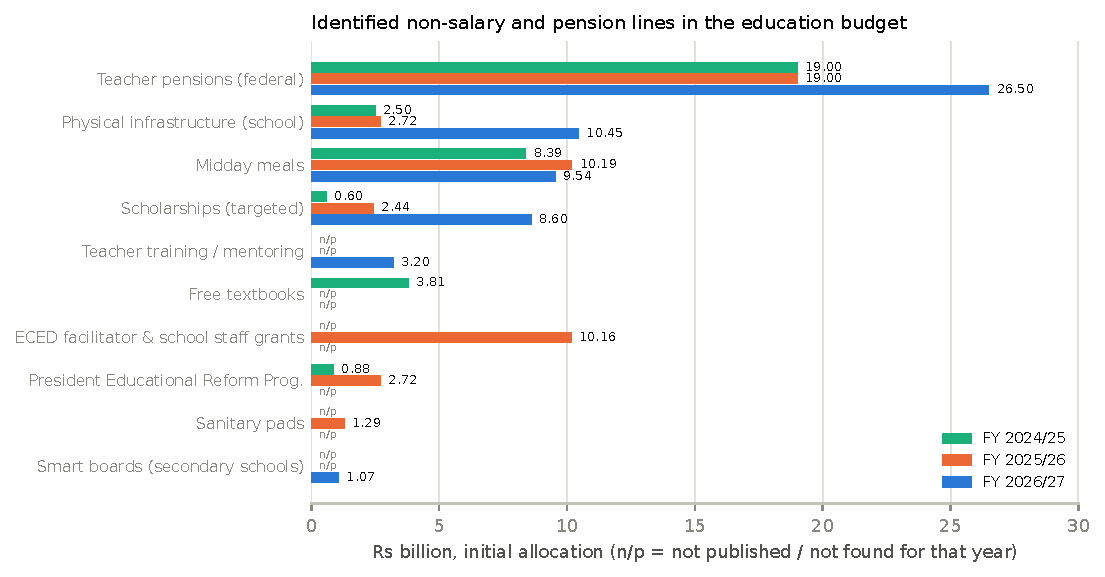
\includegraphics[width=\textwidth]{fig_programmes.pdf}
\caption{Identified non-salary lines and teacher pensions, FY~2024/25--2026/27, Rs~bn. Sources: \cite{kp2024dec,edusanjal2024b,edusanjal2025,nce2025,ratopati2026,republica_meals2026,mof2026,khabarhub2026,republica_budget2026}. The Ministry does not publish a full programme-by-programme table, so gaps reflect reporting, not zero allocation.}\label{fig:programmes}\end{figure}

\subsection{What this means for the per-student figure}
Of the Rs~34,600 allocated per community-school student in 2026/27, roughly Rs~24,000 is teacher and staff pay (applying the 69\% salary share), about Rs~2,400 is infrastructure, Rs~2,200 is school meals (concentrated on the 2.8~m youngest children), Rs~2,000 is scholarships and well under Rs~1,000 is teacher training. Trend analysis of the headline figure is therefore mostly trend analysis of the teacher wage bill divided by a shrinking number of public-school students.

\section{Data and method}\label{sec:method}
\subsection{Budget series}
Table~\ref{tab:budget} gives the initial education allocation and total federal budget for every fiscal year from 2008/09 to 2026/27. Two definitional points matter. First, after the 2017 local elections most school-education spending was re-routed as conditional grants to the 753 local governments; the Red Book ``Ministry of Education'' line fell to Rs~66.12~bn (5.17\%; the Kathmandu Post reported Rs~65.14~bn) in 2017/18 \cite{edusanjal_trend,kp2017}, while UNICEF, NCE Nepal and the Ministry of Finance report the consolidated education \emph{sector} total (federal + provincial + local conditional grants), e.g.\ Rs~126.78~bn (9.91\%) \cite{unicef2020}. This report uses the consolidated sector total throughout, so the series is comparable across the federal transition. Second, figures are \emph{initial allocations}, not actual expenditure; actual spending is normally lower, and the 2021/22 ordinance budget was later replaced \cite{nce2025}.

\begin{table}[htbp]\centering\small
\caption{Education allocation and federal budget, FY 2008/09--2026/27 (Rs billion, nominal, initial estimates)}\label{tab:budget}
\begin{tabular}{llrrrl}\toprule
FY (AD) & FY (BS) & Total budget & Education & Share (\%) & Source \\\midrule
\csname @@input\endcsname tab_budget.tex 
\bottomrule\end{tabular}
\par\smallskip\raggedright\footnotesize Notes: 2017/18 onward is the consolidated education sector (incl.\ conditional grants to provinces and local governments). 2012/13: UNICEF gives Rs~63.43~bn; NCE Table~8 gives 73.43~bn with the same 15.67\% share, which is internally inconsistent, so 63.43 is used. 2011/12: the ``17.1\% in 2011/12'' widely quoted in the press \cite{kpedit2026} corresponds to FY~2010/11 (2067/68) in the NCE/UNICEF tables; 2011/12 is 16.6\%. Minor press-vs-Red-Book differences (e.g.\ 134.19 vs 134.51 for 2018/19) are within 0.3\%.
\end{table}

\subsection{Enrolment series}\label{sec:enrol}
Grades 1--12 enrolment by school type is available from the CEHRD Flash~I reports and the Economic Survey for 2018/19 (community only) and for 2021/22--2025/26 \cite{ssdp2020,sesp2022,flash2079,flash2080,collegenp2025,kp2026es}. For 2008/09--2020/21 the only series readable for this report is the World Bank/UIS total (primary grades 1--5 plus secondary 6--12), which reconciles exactly with Flash figures where they overlap (e.g.\ 2022/23 primary 3,610,603 in both) \cite{wb_enrol}. The community-school count for those years is \emph{estimated} by applying the UIS private-enrolment share for primary to all grades \cite{wb_priv}; it is shown with an asterisk and dashed lines, and the by-government averages that depend on it should be read as indicative. The Flash~I Report 2082 (2025/26) has so far been released only as spreadsheet annexes; its figures are taken from the Economic Survey 2082/83 as reported by the Kathmandu Post \cite{kp2026es}. For FY~2026/27 the 2025/26 enrolment is used, because the 2026/27 school year is still in progress.

\begin{table}[htbp]\centering\small
\caption{School enrolment, grades 1--12, by school type}\label{tab:enrol}
\begin{tabular}{lrrrl}\toprule
School year & All students & Community & Institutional & Source \\\midrule
\csname @@input\endcsname tab_enrol.tex 
\bottomrule\end{tabular}
\par\smallskip\raggedright\footnotesize $^\ast$Estimated: total $\times$ (1 $-$ UIS private primary share) \cite{wb_priv}; for 2019/20 the UIS primary (25.4\%) and secondary (23.8\%) private shares are applied separately; for 2020/21 the 2021/22 Flash institutional share (25.9\%) is assumed. $^\dagger$UIS 2018 value missing; interpolated. 2018/19 community figure is basic 4,124,478 + secondary 1,152,674 from Flash 2018/19 as cited in \cite{ssdp2020}; the institutional column for that year is the UIS total minus that figure. 2022/23 total includes 137,527 students in religious schools, which later Flash reports count inside ``community''. Where the Economic Survey and Flash differ for the same year (e.g.\ 66.2\% vs 66.7\% community share in 2024/25) the difference is $<$1\%.
\end{table}

\subsection{Per-student measures and deflation}
Three ratios are reported for each year:
\begin{align*}
\text{(a) per enrolled student} &= \frac{\text{education sector allocation}}{\text{all grade 1--12 students}},\\
\text{(b) per community-school student} &= \frac{\text{education sector allocation}}{\text{community-school students}},\\
\text{(c) school-education per community-school student} &= \frac{\text{school-education allocation}}{\text{community-school students}}.
\end{align*}
Measure~(c) is the conceptually correct answer to ``what does the government spend per public-school student'', but a school-education sub-line is only published explicitly for 2026/27 (Rs~151.69~bn); for 2021/22, 2022/23, 2024/25 and 2025/26 the local-government education conditional grant (Rs~114.91, 121.01, 141.36 and 145.68~bn) is used as a proxy, since it is almost entirely school education \cite{unicef2022,onlinekhabar2026,kp2024dec,nce2025}. Measures~(a) and~(b) are available for all years and are used for the trend. Real values are expressed in FY~2025/26 prices using the World Bank/IMF CPI (2010 = 100), averaging the two calendar years each fiscal year spans \cite{wb_cpi}; FY~2026/27 assumes 5\% inflation. ECED/pre-primary (1.22~m children) is excluded from all denominators; including it would lower every figure by roughly 15\%.

\section{Results}\label{sec:results}
\subsection{FY 2026/27}
\begin{table}[htbp]\centering\small
\caption{Government allocation per school student, FY 2026/27}\label{tab:fy27}
\begin{tabularx}{\textwidth}{Lrrr}\toprule
Measure & Numerator (Rs bn) & Denominator (students) & Rs per student \\\midrule
\textbf{School-education allocation per community-school student} \cite{radionepal2026,kp2026es} & 151.69 & 4,383,655 & \textbf{34,604} \\
\quad excluding Rs 10.45 bn infrastructure & 141.24 & 4,383,655 & 32,220 \\
Whole education \& sports budget per community-school student & 218.30 & 4,383,655 & 49,799 \\
Whole education \& sports budget per enrolled student (all schools) & 218.30 & 7,040,825 & 31,005 \\
School-education allocation per enrolled student (all schools; a national average, not what any student receives) & 151.69 & 7,040,825 & 21,544 \\
\bottomrule\end{tabularx}
\end{table}

The best single answer is \textbf{Rs~34,600 per community-school student per year} (about US\$255 at Rs~135/\$), of which roughly 69\% is teacher and staff salaries and pensions \cite{ratopati2026}. Because the sub-sector split places university, TVET, management and sports money outside ``school education'', Rs~49,800 (the whole ministry budget per public-school student) is an upper bound.

\subsection{Trend, 2008/09--2026/27}
\begin{figure}[htbp]\centering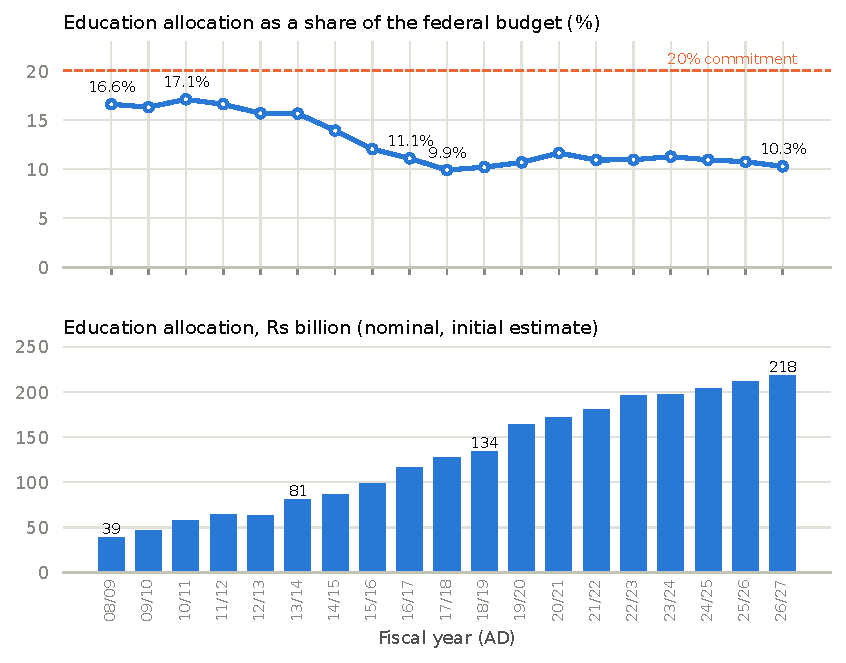
\includegraphics[width=\textwidth]{fig_budget.pdf}
\caption{Education allocation: share of the federal budget (top) and nominal amount (bottom). Sources: Table~\ref{tab:budget}.}\label{fig:budget}\end{figure}

\begin{figure}[htbp]\centering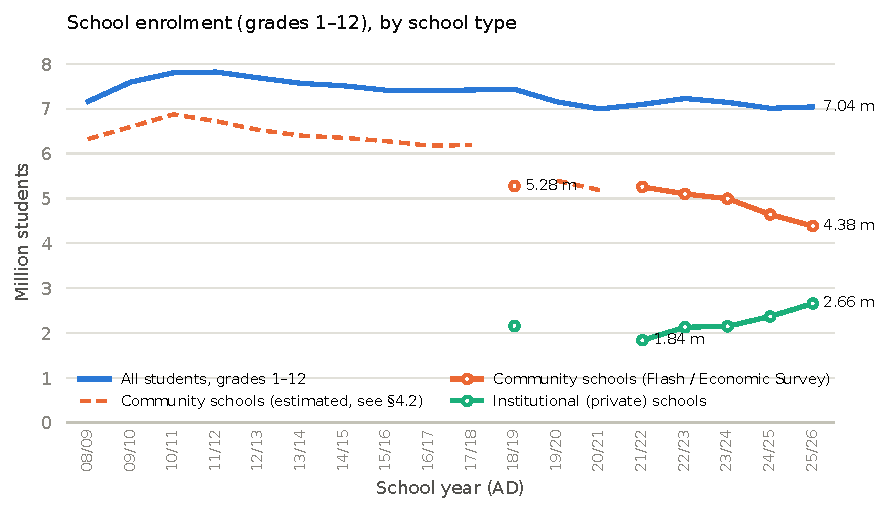
\includegraphics[width=\textwidth]{fig_enrol.pdf}
\caption{Enrolment in grades 1--12. Solid markers are Flash/Economic Survey counts; the dashed line is the estimate described in Section~\ref{sec:enrol}. Sources: Table~\ref{tab:enrol}.}\label{fig:enrol}\end{figure}

\begin{figure}[htbp]\centering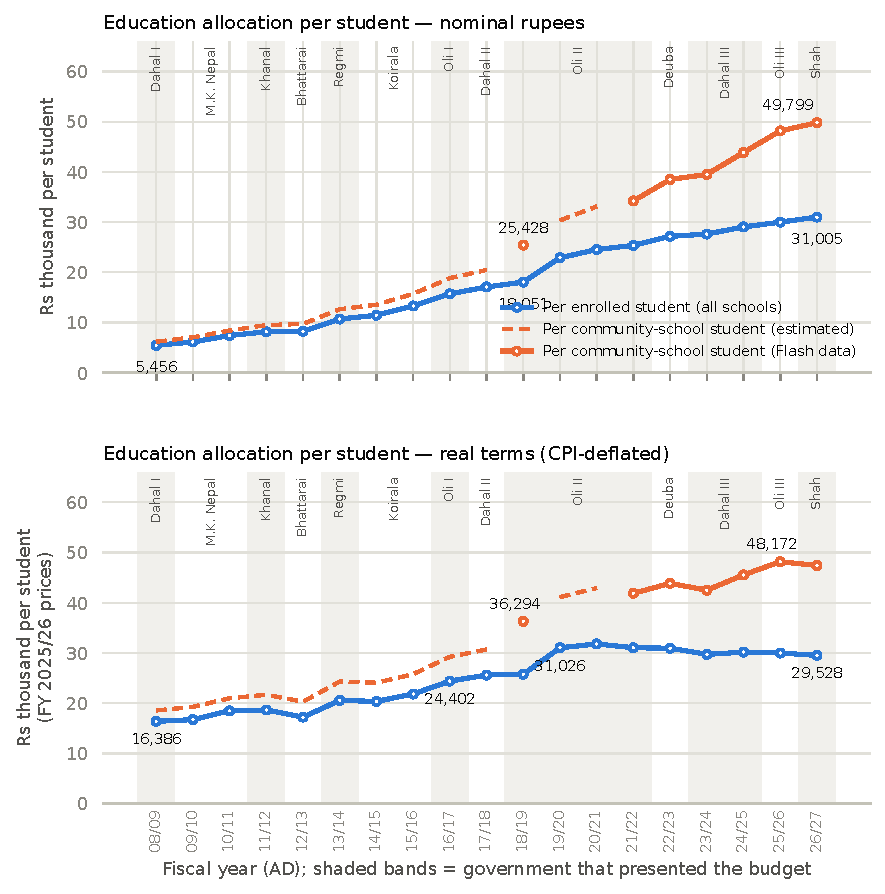
\includegraphics[width=\textwidth]{fig_perstudent.pdf}
\caption{Education allocation per student, nominal (top) and in FY~2025/26 prices (bottom). Shaded bands mark the government whose prime minister was in office when each budget was presented (Table~\ref{tab:gov}). Dashed orange segments rely on estimated community enrolment. Sources: Tables~\ref{tab:budget}--\ref{tab:enrol}, CPI \cite{wb_cpi}.}\label{fig:perstudent}\end{figure}

Three things stand out in Figures~\ref{fig:budget}--\ref{fig:perstudent}.
\begin{enumerate}[leftmargin=1.4em]
\item \textbf{Priority has halved.} Education's share of the budget fell from 16.6--17.1\% (2008/09--2011/12) to under 10\% in 2017/18 and has not recovered; 2026/27's 10.28\% is the second-lowest since then (after 10.20\% in 2018/19) \cite{kpedit2026,kp2026budget}. The nominal amount grew 5.6-fold (Rs~39.1~bn to 218.3~bn), but the total budget grew 9-fold.
\item \textbf{Real spending per student rose until 2019/20 and has been flat since.} In FY~2025/26 prices the allocation per enrolled student rose from Rs~16,400 (2008/09) to Rs~31,000 (2019/20), helped by an 8.5\% fall in total enrolment from its 2011/12 peak, and has since stayed between Rs~29,500 and Rs~31,800. The 2026/27 budget (Rs~29,500 real) is marginally below 2025/26.
\item \textbf{The rise per public-school student is a denominator effect.} Nominal allocation per community-school student roughly doubled from Rs~25,400 (2018/19) to Rs~49,800 (2026/27), and in real terms rose from Rs~36,300 to Rs~47,400. But over 2021/22--2025/26 the education budget grew 17\% nominally but \emph{fell} about 4\% in real terms, while community-school enrolment fell 17\% (5.26~m to 4.38~m) as families moved to private schools (institutional enrolment up 45\%, 1.84~m to 2.66~m) \cite{sesp2022,kp2026es}. Per-student spending in public schools is rising mainly because there are fewer public-school students, not because the state is spending more.
\end{enumerate}

\subsection{Spending by government}
Table~\ref{tab:gov} lists, for every budget, the prime minister and finance minister who presented it and the resulting per-student allocation; Table~\ref{tab:bygov} and Figure~\ref{fig:bygov} average the real figures over each government's budgets. Governments are attributed by the prime minister in office on budget day (the constitutional date, 15 Jestha / 28--29 May, applies from 2016/17; earlier budgets were presented in July--November, some by ordinance) \cite{wiki_fm,drcn2024}. The FY~2021/22 budget was issued by ordinance by the caretaker Oli government after the House dissolution and later revised by the Deuba government; it is attributed to Oli~II. No budget was presented by the Karki interim government (September 2025--March 2026); the first budget after the 5~March 2026 election, in which the RSP won 182 of 275 seats \cite{commons2026}, was presented on 29~May 2026 by Finance Minister Swarnim Wagle under Prime Minister Balendra Shah \cite{wiki_shah,ican2026}.

\begin{table}[htbp]\centering\footnotesize
\caption{Governments, budget presenters and allocation per student, FY 2008/09--2026/27 (Rs per student per year)}\label{tab:gov}
\setlength{\tabcolsep}{3.5pt}
\begin{tabular}{l>{\raggedright\arraybackslash}p{2.6cm}>{\raggedright\arraybackslash}p{2.5cm}>{\raggedright\arraybackslash}p{2.1cm}rrrr}\toprule
 & & & & \multicolumn{2}{c}{Nominal} & \multicolumn{2}{c}{FY 2025/26 prices} \\\cmidrule(lr){5-6}\cmidrule(lr){7-8}
FY & Prime minister & Finance minister & Party of PM & All students & Community & All students & Community \\\midrule
\csname @@input\endcsname tab_gov.tex 
\bottomrule\end{tabular}
\par\smallskip\raggedright $^\ast$Community-school denominator estimated (Section~\ref{sec:enrol}). ``All students'' = education sector allocation $\div$ all grade 1--12 students; ``Community'' = education sector allocation $\div$ community-school students. Sources: Tables~\ref{tab:budget}--\ref{tab:enrol}; PM/FM from \cite{wiki_fm,drcn2024,wiki_shah,commons2026}.
\end{table}

\begin{table}[htbp]\centering\small
\caption{Average real education allocation per student by government presenting the budget (Rs per student per year, FY 2025/26 prices)}\label{tab:bygov}
\begin{tabular}{lllrr}\toprule
Government & Party & Budgets (FY) & All students & Community-school \\\midrule
\csname @@input\endcsname tab_bygov.tex 
\bottomrule\end{tabular}
\par\smallskip\raggedright\footnotesize Pre-2018/19 community-school figures rest on estimated denominators. NCP = Nepal Communist Party (merged UML--Maoist Centre, 2018--2021). MC = Maoist Centre.
\end{table}

\begin{figure}[htbp]\centering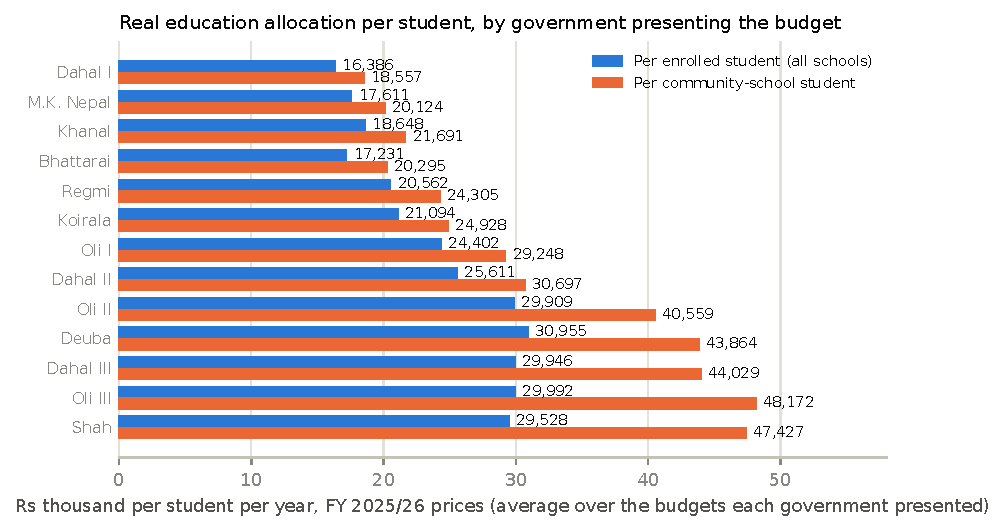
\includegraphics[width=\textwidth]{fig_bygov.pdf}
\caption{Real education allocation per student by government (average over the budgets each presented). Source: Table~\ref{tab:bygov}.}\label{fig:bygov}\end{figure}

Reading the by-government figures: the Maoist and UML governments of 2008--2012 allocated the highest \emph{share} of the budget to education (16--17\%) but, with a budget one-ninth of today's and 7.5--7.8~million students, the least per student in real terms (Rs~16,000--19,000). The Koirala (NC) and Oli~I (UML) budgets of 2014/15--2016/17 raised real spending per student by about a fifth (from Rs~20,600 in 2013/14 to Rs~24,400 in 2016/17) as the overall budget expanded after the 2015 earthquake, even while the education share fell below 12\%. The Oli~II/NCP government (2018/19--2021/22) presented the budgets in which real per-student allocation reached its present level (Rs~30,000 per enrolled student; Rs~36,000--43,000 per community-school student), a period that coincides with the federal transition and the start of the drop in community-school enrolment. Since then the Deuba (NC), Dahal~III (Maoist Centre), Oli~III (UML) and Shah (RSP) governments have each held real allocation per enrolled student at Rs~29,500--31,000: in constant prices no government since 2019/20 has materially raised education spending per student, and the 2026/27 budget continues that pattern with the second-lowest education share since 2017/18.

\section{Is this how it is measured internationally?}\label{sec:intl}
\subsection{The standard definitions}
Three conventions dominate international statistics.
\begin{itemize}[leftmargin=1.4em]
\item \textbf{UNESCO UIS / World Bank WDI.} ``Government expenditure per student is the average general government expenditure (current, capital, and transfers) per student in the given level of education, expressed as a percentage of GDP per capita'', ``calculated by dividing total government expenditure on primary education by the number of students at primary level'' \cite{wb_meta_prim}. The UIS variant used for SDG~4.5.4, ``initial government funding per student'', is general government expenditure (all tiers, current and capital) on a level of education \emph{minus international transfers to government}, divided by enrolment at that level, expressed in constant PPP dollars or as a share of GDP per capita \cite{uis_meta}. The denominator is all students at the level, public and private; the numerator is actual expenditure, by ISCED level, including transfers to private institutions and households.
\item \textbf{OECD Education at a Glance (Indicator C1).} ``Expenditure per student on educational institutions at a particular level of education is calculated by dividing total expenditure on educational institutions at that level by the corresponding full-time equivalent enrolment'', converted at GDP purchasing-power parities and also shown relative to GDP per capita \cite{oecd2023}. The OECD numerator includes public, private and international spending on institutions, and OECD countries spend on average 26\% of GDP per capita per student from primary to tertiary \cite{oecd2022}.
\item \textbf{UNICEF budget briefs} divide the consolidated education budget by the school-age population rather than by enrolment, which gives a lower figure (NPR~24,000 for Nepal in 2021/22) \cite{unicef2022}.
\end{itemize}

\subsection{How this paper's measure differs}
Table~\ref{tab:defs} sets the measure used here against the international conventions.

\begin{table}[htbp]\centering\small
\caption{Measurement conventions compared}\label{tab:defs}
\begin{tabularx}{\textwidth}{lLLL}\toprule
Dimension & This paper & UNESCO UIS / World Bank & OECD EAG C1 \\\midrule
Spending measure & Initial budget allocation & Actual expenditure & Actual expenditure \\
Sources counted & Government only & Government only (all tiers) & Public + private + international \\
Level & Grades 1--12 combined (school education sub-sector) & By ISCED level (primary, secondary) & By ISCED level \\
Students & Community-school headcount & All enrolled at the level, public and private & Full-time-equivalent, all institutions \\
Capital spending & Included (shown separately) & Included & Included \\
Pensions & Included where in the education budget & Not addressed in the definition & Not addressed \\
Normalisation & Nominal Rs; CPI-deflated & \% of GDP per capita; constant PPP\$ & PPP\$; \% of GDP per capita \\
\bottomrule\end{tabularx}
\end{table}

The choice of denominator is the substantive difference. The international statistic answers ``how much does the government spend on education at this level, per child enrolled at this level, whoever educates them''; it treats a country where a third of children are privately educated at their parents' expense as spending less per child. The measure in this paper answers ``how much does the state spend per child it actually educates'', which is the right question for judging the resourcing of public schools, and it is the one Nepal's Ministry and ADB use when they quote the conditional grant per community-school student (NPR~13,809 in FY2019) \cite{adb2021}. Both are legitimate; they should not be compared with each other. Two further differences matter less in Nepal's case: allocation versus expenditure (actual spending runs below allocation, so the figures here are upper bounds), and headcount versus full-time-equivalent (school pupils count as one FTE each in almost all countries).

\subsection{Nepal on the international convention}
To place Nepal against its neighbours the paper re-expresses the 2026/27 allocation on the UIS convention: school-education allocation Rs~151.69~bn $\div$ all 7,040,825 students $=$ Rs~21,544, which is \textbf{9.7\% of GDP per capita} (Rs~222,841, derived from the provisional 2025/26 GDP of Rs~6,600,099~m and a population of 29.6~m \cite{nrb2026,wb_pop}). The whole education and sports budget per enrolled student is Rs~31,005, or 13.9\% of GDP per capita; the public-school measure, Rs~34,604, is 15.5\%. The WDI's own last observation for Nepal, from actual expenditure, is 12.4\% for primary and 10.5\% for secondary (2015) \cite{wb_xpd}.

\begin{figure}[htbp]\centering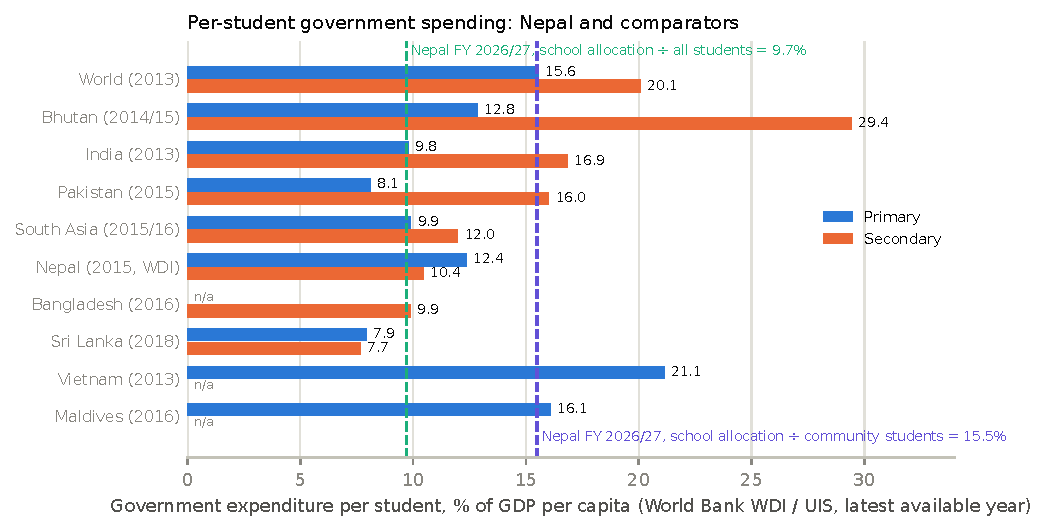
\includegraphics[width=\textwidth]{fig_intl.pdf}
\caption{Government expenditure per student as a share of GDP per capita, latest WDI observation per country (actual expenditure, all enrolled students) \cite{wb_xpd}, with Nepal's FY~2026/27 allocation-based figures marked. Years differ by country and the regional series is stale; treat as orders of magnitude.}\label{fig:intl}\end{figure}

Figure~\ref{fig:intl} shows that, on a like-for-like basis, Nepal spends about as much per student relative to its income as South Asia as a whole (9.9\% primary, 12.0\% secondary) and less than the world average (15.6\% and 20.1\%); Bhutan (12.9\% and 29.4\%) and India at the secondary level (16.9\%) spend more, Sri Lanka and Pakistan at the primary level less \cite{wb_xpd}. On the broader aggregates Nepal's education spending is 3.7\% of GDP and 10.8\% of government expenditure (2024--25), compared with 2.9\% and 11.3\% for South Asia and 3.6\% and 14.0\% for the world \cite{wb_xpd}; the 2026/27 allocation of Rs~218.30~bn is 3.1\% of the IMF's projected 2026/27 GDP of Rs~7,148~bn \cite{imf2026}. Nepal therefore spends a comparatively high share of its (small) GDP on education but a below-average share of its budget, and the per-student result is middling for the region. The comparison should be read loosely: the WDI per-student series ends in 2013--2018 for every South Asian country, and the Nepal figure here is an allocation for grades 1--12 combined rather than audited expenditure by level.

\section{Limitations}
\begin{enumerate}[leftmargin=1.4em]
\item \textbf{Allocations, not expenditure.} All budget figures are initial estimates; actual spending is typically 80--90\% of allocation and revised budgets (notably 2021/22) differ.
\item \textbf{Sector definition.} Figures from 2017/18 include provincial and local conditional grants but not local governments' own-source spending on schools, which is small but growing.
\item \textbf{Estimated community enrolment before 2018/19.} The DoE Flash reports for 2008/09--2017/18 exist but could not be retrieved; the UIS private-primary share was applied to all grades, which probably overstates the community count (private shares are higher in secondary grades) and therefore understates per-community-student spending in those years by perhaps 5--10\%.
\item \textbf{Year matching.} Nepal's fiscal year (mid-July) and school year (mid-April) do not coincide; the school year that begins three months before each budget is used. FY~2026/27 uses 2025/26 enrolment.
\item \textbf{Religious schools} (1,387 schools, c.\ 137,000 students) are counted inside ``community'' in most sources; this affects per-student figures by under 3\%.
\item \textbf{Deflation.} Fiscal-year deflators average two calendar-year CPI values; 2026/27 assumes 5\% inflation. GDP-based or education-specific deflators would give somewhat different real series.
\item \textbf{Composition data are partial.} The Ministry publishes shares by sub-sector, tier and economic nature but no complete programme table; the line items in Section~\ref{sec:composition} are those reported in the budget speech and the press, and some (e.g.\ the Rs~133.8~bn teacher-salary figure) come from analysts' re-classifications that cannot be reconciled exactly with the Ministry's 68.98\% salary share.
\item \textbf{International comparison} uses an allocation for grades 1--12 against WDI expenditure figures by level from 2013--2018, and a derived GDP per capita; it indicates orders of magnitude only.
\item \textbf{Government attribution} by the prime minister on budget day ignores coalition composition (e.g.\ NC finance minister Prakash Sharan Mahat presented the 2023/24 budget under Maoist PM Dahal) and the fact that budgets are largely driven by salary commitments inherited from predecessors.
\end{enumerate}

\bibliographystyle{unsrtnat}
\renewcommand{\bibfont}{\small}
\bibliography{refs}
\end{document}
